%%%%%%%%%%%%%%%%%%%%%%%%%%%%%%%%%%%%%%%%%%%%%%%%%%%%%%%%%%%%%%%%%%%%%%%%%%%%%%%

\chapter{INTRODUCTION}\label{ch:intro}

The Satellite Control Center (CCS) at the National Institute for Space Research (INPE) currently operates the following satellites: the Data Collection Satellite family (SCD), made of two satellites SCD1 and SCD2; and the China-Brazil Earth Resources Satellite (CBERS) family, currently operating the fifth and the sixth satellites in the family, CBERS-4 and CBERS-4A.
Each satellite pass by INPE's ground stations, a period called overpass in which CCS receives satellite health via telemetry data, and chooses to send commands via telecommands to control the satellite.
This entails maintenance and operation capabilities, as the orbit and equipment health need to be measured and adjusted for each satellite, with decisions being made by engineering~\cite{AzevedoAmbr:2010:ArSaTe}.

Telemetry data are composed of on-board sensors and equipment health measures gathered by the On-Board Computer (OBC), like battery current, system voltage, whether a given equipment is active or not, and any other data that is necessary for the satellite operators to execute the operation procedures~\cite{larsonSpaceMissionAnalysis1999}.
These data need to be stored for the entire life cycle of the satellite, as long-lived satellites that work for decades generate a considerable amount of data, which must be analyzed by the operators.
For the SCD family, SCD1 has been operational for 25 years, even if in an degraded state, and keep generating data of about 7GB per year, with an average 8 station passes per day.

However SCD1 is only a small satellite, tracking only about 100 telemetry points, and more complex satellites like the ones from the CBERS family will track over 4 thousand telemetries at once.
With the future launch of the Amazônia-1 satellite, INPE will be operating 5 satellites at once (CBERS-4, CBERS-4A, AMZ-1, SCD1 and SCD2), which generates pressure to the operation activities~\cite{JulioFoAmbrFerrLour:2017:ChImSp}.

\autoref{fig:totaldatagen} shows a simple statistic of the expected volume of telemetry data being handled by CCS since the launch of SCD1 in 1993, and with the added volume of the CBERS and AMZ programs.
This assumes a constant rate for the telemetry data, however closely tracks the average raw engineering data generation.
The majority of these data are not available for analysis, as every few years it is archived on tapes by INPE, and thus the operators in general only deal with data that goes a few months back for each satellite, and not with the full volume for each.

\begin{figure}[!hb]
  \caption{Historic telemetry data generation}\label{fig:totaldatagen}
  \vspace{4mm}
  \begin{center}
    \resizebox{13cm}{!}{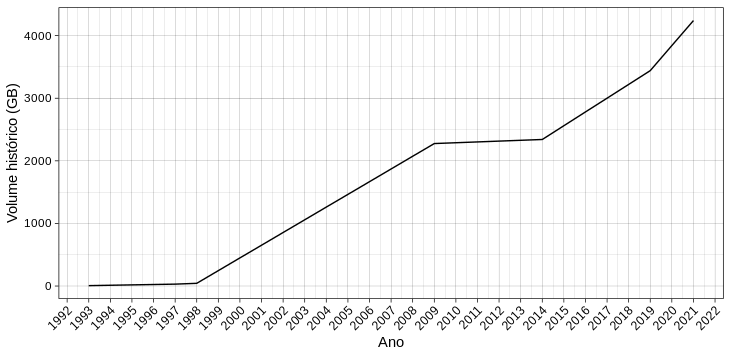
\includegraphics{Figuras/VolumeToYear.png}}
  \end{center}
  \vspace{2mm}
  \legenda{Estimated telemetry data volume generated by INPE since the first satellite launch.}
  \FONTE{Author}
\end{figure}

It is necessary to be careful so that the data do not become ``\textit{dark data}'', a concept meaning data is not available for all users that could benefit from it~\cite{heidornSheddingLightDark2008}.

These data would classify as Big Data, as they represent a considerable volume, are constantly generated, have differing formats, their analysis is of high value and there is some uncertainty as to quality of the data, as not only communication problems occurs, the natural degradation of equipments can mislead users.
These characteristics are encapsulated by the five Vs of Big Data: Volume, Variety, Velocity, Value and Veracity~\cite{kacfahemaniUnderstandableBigData2015}.

Even if all of these data were available for the satellite operators at once, there is still the problem of querying a database with terabytes of data, in which queries over a long timespan or over too many telemetries would not be trivial and could take hours to complete.

In order to make the operator work feasible, database systems are deployed that enable the visualization of telemetry points over time, get the data in a specific format and execute query operations on it.
However, to go beyond previously defined queries and visualizations, these systems require the use of a query language, which further requires operator training and experience to know what and how to ask, and how to format the result as to make it understandable for other mission members.
This is further complicated by each satellite and telemetry format being different: it is necessary to understand how each individual spacecraft behaves and how the telemetries communicate that behavior to perform analysis on the data \cite{uhligSpacecraftOperations2015}).

An efficient solution is to create a Data Warehouse (DW) suited to the analysis of the data, tailored to answer the most relevant and frequent domain questions about the data, which is extended by implementing On-Line Analytical Processing (OLAP), that aims to enable the exploratory analysis of the data in a fast and user-centric way \cite{hanDataMiningConcepts2011,viswanathanUsercentricSpatialData2014}.
This has been proposed and implemented for the satellite operations and ground segment with good results \cite{adamskiDataAnalyticsLarge2016,yvernesCopernicusGroundSegment2018}.

In order to allow for fast OLAP operations on a Data Warehouse, the data cube has been created as a query operator to pre-compute and store multidimensional aggregations, enabling users to perform multidimensional analysis on-line, and have since played an essential role in creating stable solutions for Data Warehouses \cite{grayDataCubeRelational1996}.
However, it is often necessary to materialize a part of the data cube beforehand, as this provides a way to pre-compute and store multi-dimensional aggregates and operations, enabling for multi-dimensional analysis to be performed on the fly (on-line).

A data cube is constituted of dimensions and measures: dimensions relate to the constituent attributes of the data, determining its context; while measures are the calculated relationships between the dimensions.
Each dimension can have different values at different data points, the number of distinct values in the dimension is defined as the dimension's cardinality (denoted by \(\mathcal{C}_i\) for a dimension \(i\)).
The data cube is based on the tuples of the data, as the cube operator will generalize groups of values in each dimension as part of the concept of aggregate cells that have those values in those dimensions, thus generating the cells of the cube \cite{hanDataMiningConcepts2011}.
The tuples can be of any value, and the distribution of these values within a dimension is called the skew: if values are repeated too often (\(\mathcal{C}_i \ll n\), for a dimension \(i\)), the dimension is said to have a high skew.

The cells that are related to some dimensions form a cuboid: one of the possible subsets of the combination of dimensions, with a resulting measure computed between the data, resulting in the relationship between those dimensions.
These cuboids will have the size of the cardinalities of each constituent dimensions multiplied, and they can be 0-dimensional up to \(n\)-dimensional, for a number of \(n\) dimensions.

For that reason it is necessary to choose an appropriate data cube computation algorithm, of which several have been proposed to partially, or fully, materialize a data cube, like \cite{dokaBrownDwarfFullydistributed2011,dongxinCCubingEfficientComputation2006,liSemiClosedCubeEffective2005,liHighdimensionalOLAPMinimal2004,xinComputingIcebergCubes2007}.
To say that a cube is fully materialized means that all the \(0\)-dimensional to \(n\)-dimensional cuboids have been pre-computed, with partial materialization pre-computing some of those cuboids, and no materialization pre-computing $0$ cuboids.

However, one of the main limitations that these algorithms face is keeping system memory consumption low: as it is a $2^d$ storage operation, with $d$ being the number of dimensions used, it is often not possible to fully materialize the data cube, making partial materialization strategies necessary.

The work of \cite{liHighdimensionalOLAPMinimal2004} presents Frag-Cubing, an algorithm to materialize the minimal data cube necessary to answer queries with few dimensions, while using less memory to answer the queries that need more dimensions.
Frag-Cubing uses an inverted index schema that excels at answering queries from data that has a high skew: data that focuses on values that are repeated often are compressed into fewer indices, that can then be used to more efficiently answer queries.
In Frag-Cubing, each attribute value of a tuple is associate with $1-n$ tuple identifiers (TID).
Point queries with two or more attribute values are answered by intersecting tuple identifiers of these attribute values.
%Frag-Cubing only implements equal and sub-cube query operators, limiting the amount of operations that can be performed.

Though the choice of the data cube construction algorithm can reduce the memory and storage space usage of the data warehouse, it is still necessary to adapt the data into schemas to further reduce the dimensionality and improve the organization of the data.

\section{Research Objectives}\label{ch:intro:obj}

%- Ao invés de usar características, utilizar as distribuição estatística dos valores de telemetria do satélite para
%Criar uma arquitetura básica de cubo de dados para representação da distribuição dos valores de telemetrias ao longo de uma missão, para facilitar a análise e consulta do estado do satélite pelos engenheiros de satélite.

The goal of this thesis is to create a data cube base architecture to represent satellite telemetry data along a mission, using the distribution of the telemetry values to ease analysis and querying of the satellite's state by satellite engineers.

Specific objectives of this work include:

\begin{itemize}[noitemsep]
  \item To test two approaches of reducing the memory usage of the Frag-Cubing algorithm, with the goal of reducing implementation requirements for a data warehouse based on a data cube, using the telemetry value distribution of satellite telemetry data.
It will use the information gathered by analysing the satellite telemetries to select and optimize queries, taking into account the high dimensionality, high number of tuples, high skew and high cardinality of the base data.
  \item To probe whether the use of inverted index compression via list intervals can improve the memory consumption and query response times for the Frag-Cubing algorithm.
  With the results being evaluated against the Frag-Cubing original implementation, it will be possible to know when to use each of the alternatives and decide for which dimensions and/or kinds of data they are applicable.
\end{itemize}

\section{Method}\label{ch:intro:method}

To evaluate whether the approaches are useful for a satellite operator, first an algorithm will be implemented to find relationships between telemetries and then this will be evaluated with an experienced satellite operator as to how useful it is.
Then the queries selected will be filtered, and an approach of pre-processing the input data will be executed, were the data are filtered to only the dimensions that will be queried and then evaluated as to whether that improves query response times and memory consumption for each type of query.

This will be experimentally evaluated on data from one of INPE's satellite, notably SCD2, for which the Satellite Control Center (CCS) has allowed the use of over 4 years of satellite telemetry data, totalling over $24GB$ of raw data and associated documentation, with 135 telemetries being tracked.

\section{Contributions}\label{ch:intro:contrib}

This work aims to use open source software to define an improved data cube algorithm, and thus it is expected to save money and time for space organizations that operate satellites and need to implement their own telemetry data analysis structures to analyse data.
This work is being performed using open source software, open literature and aims to publish the satellite telemetry data used as a case study for others in the end.
Furthermore, all analyses and experiments are designed to be reproducible via open source software repository.

For the Frag-Cubing family of algorithms, this also shows that simpler strategies can be used to improve memory consumption and query response times, first by simple pre-processing of frequent queries and then by changing the inverted index compression strategy of the algorithm to drastically reduce memory usage.

\section{Document Structure}\label{ch:intro:org}

The remainder of this documented is structured as follows:

\begin{itemize}[noitemsep]
  \item{Chapter 2}: Presents the theoretical background on satellite operations, Data Warehouse, Big Data and Data Cube approaches necessary for the understanding of this work;
  \item{Chapter 3}: Related works in the literature will be presented and reviewed, as well as data cube concepts close to this one, and how other satellite operators are solving these problems with what technologies;
  \item{Chapter 4}: Presents the method, the case study experimental setup with the SCD2 satellite and showcases the sample data warehouse-based architectural vision for this work and operation activities;
  \item{Chapter 5}: Presents the Query Partitioning algorithm, the case study experimental setup with the SCD2 satellite, and the results of trying to filter the data by the query related dimensions;
  \item{Chapter 6}: Presents the IntervalFrag algorithm and the experimental validation, with an analysis of replacing Frag-Cubing's inverted index architecture;
  \item{Chapter 7}: Presents a critical analysis of the results, where each algorithm is better suited and where they excelled or had drawbacks;
  \item{Chapter 8}: Concludes the thesis, summarizing the usefulness of the results and future work that can be discussed from them.
\end{itemize}

